\subsection{Towards Ductile Fracture}
\subsectioncover

\begin{frame}
  \vspace{-1.5em}
  \begin{columns}
    \begin{column}{0.2\textwidth}
      \vspace{-1em}
      \begin{figure}
        \centering
        \begin{subfigure}{\textwidth}
          \centering
          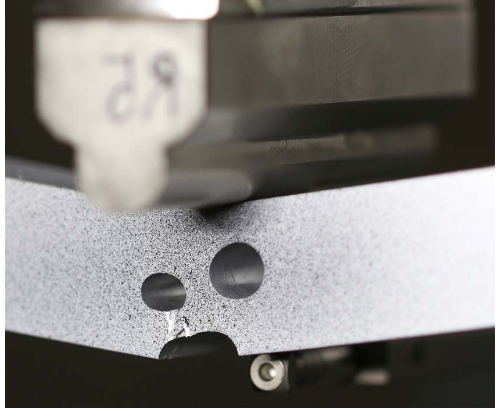
\includegraphics[width=\textwidth]{Chapter345/figures/3pb_real_crack}
        \end{subfigure}
        \begin{subfigure}{\textwidth}
          \centering
          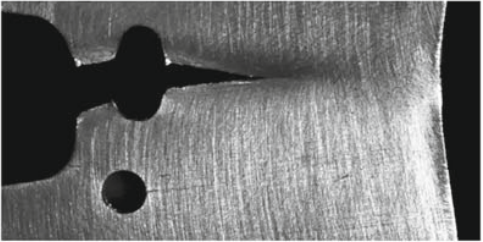
\includegraphics[width=\textwidth]{Chapter345/figures/SFC_schematics}
        \end{subfigure}
        \begin{subfigure}{\textwidth}
          \centering
          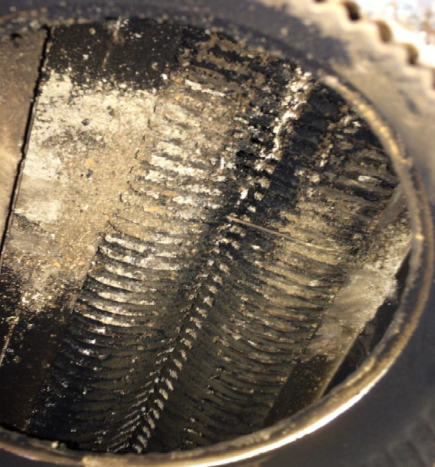
\includegraphics[width=\textwidth]{Chapter1/figures/spallation}
        \end{subfigure}
      \end{figure}
    \end{column}
    \begin{column}{0.8\textwidth}
      \vspace{1em}
      
      There exist many approaches to modeling plasticity in the context of phase-field fracture \cite{alessi_gradient_2014, alessi_gradient_2015, alessi_coupling_2018, ambati_phase-field_2015, ambati2016phase, miehe_phase_2016, borden2016phase, borden_phase-field_2017}.
      
      \bigskip
      \pause
      
      How to best design the coupling between plasticity and fracture remains an open question. Some challenges/issues:
      \begin{itemize}
        \item Fracture tends to propagate along the plastic zone.
              \pause
        \item Most existing models
              \begin{itemize}
                \item are not variational,
                      \pause
                \item require re-calibration of material parameters,
                      \pause
                \item result in regularization-dependent response.
                      \pause
              \end{itemize}
        \item How much plastic dissipation contributes to fracture evolution?
              \pause
        \item How much plastic dissipation converts to heat generation?
      \end{itemize}
      
      \bigskip
      \pause
      
      \begin{block}{}
        \centering
        \vspace{1em}
        All of the issues above can be addressed by the proposed framework \\
        (with proper constitutive choices).
        \vspace{1em}
      \end{block}
    \end{column}
  \end{columns}
\end{frame}

\begin{frame}
  \begin{block}{}
    \begin{align*}
      L = \int\limits_{\body_0} \left[ \dot{\psi}^e + {\psi^e}^* + (1-\tqf)\dot{\psi}^p + \tqf {\psi^p}^* + \dot{\psi}^f + {\psi^f}^* - T\dot{s} - \chi \right] \diff{V} - \mathcal{P}^\text{ext}, \\
      \text{subject to } \bfL(\bfZ) \dot{\bfZ} = \bs{0}.
    \end{align*}
  \end{block}
  
  \only<1>{
    \begin{columns}[T]
      \begin{column}{0.5\textwidth}
        Option 1 (Compressible Neo-Hookean):
        \begin{align*}
          \psi^e               = & \ g^e \psi^e_\activepart + \psi^e_\inactivepart,                                                              \\
          \psi^e_\activepart   = & \ \mathbb{H}_1(J)\left\{ \dfrac{1}{2}K\left[ \dfrac{1}{2}(J^2-1) - \ln(J) \right] \right\}                    \\
                                 & \ + \dfrac{1}{2}G\left( \overbar{\bfC}:{\bfC^p}^{-1} - 3 \right),                                             \\
          \psi^e_\inactivepart = & \ \left( 1-\mathbb{H}_1(J) \right) \left\{ \dfrac{1}{2}K\left[ \dfrac{1}{2}(J^2-1) - \ln(J) \right] \right\}. 
        \end{align*}
      \end{column}
      \begin{column}{0.5\textwidth}
        Option 2 (Hencky):
        \begin{align*}
          \psi^e               & =  g^e \psi^e_\activepart + \psi^e_\inactivepart,                                     \\
          \psi^e_\activepart   & = \dfrac{1}{2} K \macaulay{\tr(\strain^e)}_+^2 + G \dev{\strain^e} : \dev{\strain^e}, \\
          \psi^e_\inactivepart & = \dfrac{1}{2} K \macaulay{\tr(\strain^e)}_-^2,                                       \\
          \strain^e            & = \frac{1}{2} \ln\left( \bfC^e \right).                                               
        \end{align*}
      \end{column}
    \end{columns}
  }
  
  \only<2>{
    \begin{columns}[T]
      \begin{column}{0.33\textwidth}
        Option 1 (Linear hardening):
        \begin{align*}
          \psi^e               = & \ g^e \psi^e_\activepart + \psi^e_\inactivepart,                                                              \\
          \psi^e_\activepart   = & \ \mathbb{H}_1(J)\left\{ \dfrac{1}{2}K\left[ \dfrac{1}{2}(J^2-1) - \ln(J) \right] \right\}                    \\
                                 & \ + \dfrac{1}{2}G\left( \overbar{\bfC}:{\bfC^p}^{-1} - 3 \right),                                             \\
          \psi^e_\inactivepart = & \ \left( 1-\mathbb{H}_1(J) \right) \left\{ \dfrac{1}{2}K\left[ \dfrac{1}{2}(J^2-1) - \ln(J) \right] \right\}. 
        \end{align*}
      \end{column}
    \end{columns}
  }
\end{frame}
